\documentclass[a5paper,onecolumn,final,10pt]{memoir}

% -------- %
% Preamble %
% -------- %

\usepackage[stretch=10]{microtype}
\usepackage[utf8]{inputenc}
\usepackage[british]{babel}
\usepackage{csquotes}

%\usepackage{CJKutf8}

\usepackage{times}
\usepackage{courier}
\usepackage[T1]{fontenc}
% Greek letters %
\DeclareUnicodeCharacter{3C0}{\pi}

% Misc %
\DeclareUnicodeCharacter{2211}{\sum}
\DeclareUnicodeCharacter{222B}{\int}

%\DeclareUnicodeCharacter{2715}{\times}
\DeclareUnicodeCharacter{00D7}{\times}

\DeclareUnicodeCharacter{221A}{\sqrt}
%\DeclareUnicodeCharacter{221A}{\times}

\DeclareUnicodeCharacter{221E}{\infty}

\DeclareUnicodeCharacter{221D}{\propto}

\DeclareUnicodeCharacter{2260}{\ne}
\DeclareUnicodeCharacter{2264}{\le}
\DeclareUnicodeCharacter{2265}{\ge}

\DeclareUnicodeCharacter{227A}{\prec}
\DeclareUnicodeCharacter{227B}{\succ}
\DeclareUnicodeCharacter{227C}{\preceq}
\DeclareUnicodeCharacter{227D}{\succeq}

\DeclareUnicodeCharacter{2282}{\subset}
\DeclareUnicodeCharacter{2283}{\supset}
\DeclareUnicodeCharacter{2286}{\subseteq}
\DeclareUnicodeCharacter{2287}{\supseteq}

\DeclareUnicodeCharacter{2228}{\vee}  % \lor
\DeclareUnicodeCharacter{2227}{\wedge}  % \land
\DeclareUnicodeCharacter{222A}{\cup}
\DeclareUnicodeCharacter{2229}{\cap}

\DeclareUnicodeCharacter{2200}{\forall}
\DeclareUnicodeCharacter{2203}{\exists}

\DeclareUnicodeCharacter{22C5}{\cdot}

% Arrows %
\DeclareUnicodeCharacter{21D0}{\Leftarrow}
\DeclareUnicodeCharacter{2190}{\leftarrow}
\DeclareUnicodeCharacter{2194}{\leftrightarrow}

\DeclareUnicodeCharacter{00B9}{^{-1}}

\DeclareUnicodeCharacter{2208}{\in}

%\DeclareUnicodeCharacter{2248}{\approx}
%\DeclareUnicodeCharacter{2249}{\napprox}



% Greek letters %
\DeclareUnicodeCharacter{03C3}{\sigma}
\DeclareUnicodeCharacter{03B8}{\theta}
\DeclareUnicodeCharacter{03C1}{\rho}

\usepackage[svgnames]{xcolor}
\usepackage{graphicx}

\usepackage{amsmath}
%\usepackage{amssymb}
%\usepackage{amsfonts}
%\allowdisplaybreaks[3]
%\usepackage{amsthm}
%\usepackage{mathtools}
\usepackage{siunitx}

\usepackage{enumitem}

\newcommand{\eqv}{\mathrel{\mkern3mu\Leftrightarrow\mkern3mu}}
\newcommand{\imp}{\mathrel{\mkern3mu\Rightarrow\mkern3mu}}

\usepackage{tikz}
\usetikzlibrary{shapes,arrows,positioning,calc,decorations,arrows.meta}
\usepackage{tikz}
\usetikzlibrary{shapes,arrows,positioning,calc,decorations,arrows.meta,backgrounds}

%\tikzset{
%	warningsign/.pic={
%		\node[regular polygon sides=3,draw,] () {};
%	}
%}

\newcommand\warningsign{
	
\begin{tikzpicture}[baseline={0.95cm}]
		\node[
			regular polygon,regular polygon sides=3,
			draw,line width=4pt,
			rounded corners=4pt,
			font={\Huge\bfseries},
%			xshift=1cm,
			minimum width=1.5cm,
		] (a) {!};
	\end{tikzpicture}
}

\newcommand\warningbox[1]{
	\noindent
	\begin{tikzpicture}[framed,background rectangle/.style={draw,thick,rounded corners=1pt}]
		\node[
			regular polygon,regular polygon sides=3,
			draw,line width=4pt,
			rounded corners=4pt,
			font={\Huge\bfseries},
%			xshift=1cm,
			minimum width=1.5cm,
		] (sign) {!};

%		\node[
%			draw,thick,
%			rectangle,rounded corners=1pt,
%			text width=\textwidth,align=left,
%		] (a) {\warningsign};

%		\node[above right=3.5mm and 0cm of sign] {asd};
		\node[
%			above right=-4mm and 1cm of sign.north,
			right=1cm of sign.north,
			anchor=north west,
			align=left,
			text width=0.8\textwidth
		] {#1};
	\end{tikzpicture}
}

\definecolor{linkblue}{HTML}{0066cc}
\usepackage[
	hidelinks,  % Tirar as cores dos links
	unicode,
	colorlinks=false,
	linkcolor=MidnightBlue,
	citecolor=Green,
	urlcolor=linkblue,
]{hyperref}

\usepackage[backgroundcolor=yellow!50,textsize=tiny]{todonotes}



% ----- %
% Style %
% ----- %

\setlrmarginsandblock{1.5cm}{*}{*}
\setulmarginsandblock{3cm}{*}{1.2}
\checkandfixthelayout

\chapterstyle{plain}
%\cftsetindents{chapter}{1.5em}{2.3em}
%\renewcommand\cftchapterfont{\normalfont}
%\renewcommand\cftchapterleader{\cftdotfill{\cftsectiondotsep}}
%\renewcommand\cftchapterpagefont{\normalfont}
%\renewcommand\cftchapterafterpnum{\par\vskip-10pt}
\counterwithout{section}{chapter}

\setsubsubsecheadstyle{\itshape}

\OnehalfSpacing



% -------- %
% Document %
% -------- %

\newcommand\machinename%
%	{SNX-800B Type 5}
%	{STR-800B \textsf{\textit{Super}}}
	{\textsf{STR-800B \textit{Super}}}

\newcommand\companyname%
%	{Aperture Science\,\copyright}
	{Jikan Kei Corp.\,\copyright}



\begin{document}

\frontmatter

\begin{titlingpage}
\calccentering{\unitlength}
\begin{adjustwidth*}{\unitlength}{-\unitlength}
	\centering
	
	\vspace*{4\baselineskip}
	
	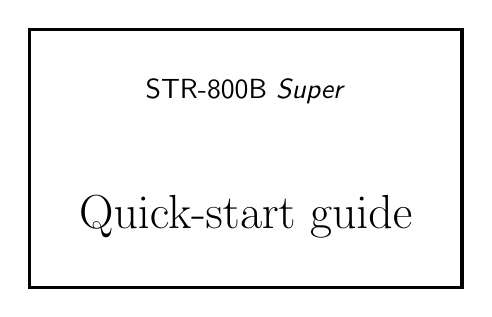
\begin{tikzpicture}
		\node[rectangle,draw,very thick,inner sep=18pt,align=center] {
			{\HUGE \machinename} 
			\\[32pt] 
			{\LARGE Quick-start guide}
		};
	\end{tikzpicture}
	
	\vfill
	
	{\footnotesize \companyname \\ Não tenho japonês instalado :(}
\end{adjustwidth*}
\end{titlingpage}



\thispagestyle{empty}

\begin{footnotesize}
\noindent
This is a quick-start guide to your \machinename\ time-computing machine. 
Please ensure you have thoroughly read and understood the User Manual and the Warranty Disclaimer before attempting to utilize the machine. 
\companyname\ is not responsible for any damages resulting from improper use of the time jump facilities of this machine. 
\todo{Meter warnings, disclaimers, etc, tipo “please always ensure your program does not contain any causality-breaking closed timelike loops”}

~

\warningbox{Example warning box. This product is without the implied warranty of MERCHANTABILITY or FITNESS FOR A PARTICULAR PURPOSE. \\[4pt] \textbf{\textsf{UNDER NO CIRCUMSTANCES SHOULD YOU COISO!}}}
\end{footnotesize}



\clearpage
\renewcommand\cftchapterfont{\ttfamily}
\renewcommand\cftchapterleader{\ttfamily\cftdotfill{.}}  % Bué intuitivo, escuta
\renewcommand\cftchapterpagefont{\ttfamily}
%\show\tableofcontents
\tableofcontents*



\mainmatter

\section{Introduction}

%Congratulations of being the proud owner 



\clearpage
\section{The Machine Language}

The following is a quick-reference guide to \machinename\ assembly language. Please use ONLY the officially licensed assembler programs by \companyname\ (ensure you have been supplied with all 9 (nine) floppy diskettes for installation of the assembler). 

%The CPU word size is 8 bits.

Quick facts:
\begin{itemize}[nosep]
	\item 8-bit word size, 16-bit address space. 
	\item 0.66\,MHz clock speed. 
	\item Four general purpose word registers.
	\item Six-word stack. 
	\item Time jumps of up to 200 clock cycles in any direction.\footnotemark
	\item Memory-mapped IO. 
	\item Big endian. 
\end{itemize}
\footnotetext[1]{Note: for jumps of over 80 clock cycles an upgraded SPS-3-6000 power supply with at least 6\,kW of peak power output must be purchased. \textbf{Serious damage may occur if you attempt to use these operations without sufficient power!}}

\subsection*{CPU registers}

The CPU has 4 (four) general purpose word-sized registers \texttt{A}, \texttt{B}, \texttt{C}, and \texttt{D}. 
These registers can be given as operands wherever an absolute memory address is expected. 

Furthermore, one stack pointer and one flag register are available. 
The flag register cannot be written to (except as a side-effect of arithmetic and comparison operations), 
%and the stack pointer cannot be read or written except by the \texttt{CAL}, \texttt{RET}, \texttt{PUS}, 
and the stack pointer is altered by the \texttt{CAL}, \texttt{RET}, \texttt{PSH}, \texttt{POP} instructions 
(besides being able to be read and written as a general purpose register). 

16-bit addresses are read and stored as two words in big-endian order: \texttt{\%llhh}. 
In order to perform 16-bit arithmetic, you must process the two words manually 
(mathematical subroutines can be purchased for as low as \$799 for non-commercial use, please contact your sales representative). 

Finally, the 16-bit program counter can be modified by jump, branching, and subroutine instructions. 

\subsection*{Addressing modes}

The following addressing modes are available:

\begin{itemize}[nosep]
	\item Register (\texttt{\%a}): addresses a named register. 
	\item Immediate (\texttt{\#ff}): represents a literal value. 
	\item Absolute (\texttt{\#llhh}): the memory address $\texttt{ll}+2^8\texttt{hh}$. 
	\item Indirect (\texttt{\#llhh}): the address stored at memory address $\texttt{ll}+2^8\texttt{hh}$. 
\end{itemize}

\subsection*{List of instructions}

The following is a quick-reference list of instructions. 

\subsubsection*{Memory management}

\noindent\texttt{MOV src dst} \quad Set word at \texttt{dst} to contents of \texttt{src}. 

\subsubsection*{Arithmetic}

\noindent\texttt{ADD src dst} \quad Set word at \texttt{dst} to $\texttt{src}+\texttt{dst}$. Set carry flag on overflow.  

\noindent\texttt{SUB src dst} \quad Set word at \texttt{dst} to $\texttt{src}-\texttt{dst}$. Set carry flag on underflow. 

\noindent\texttt{MUL src dst} \quad Set word at \texttt{dst} to $\texttt{src}×\texttt{dst}$. Set carry flag on overflow. 

\subsubsection*{Comparison}

\noindent\texttt{CMP src dst} \quad If $\texttt{src}>\texttt{dst}$ set carry flag. If $\texttt{src}=\texttt{dst}$ set zero flag. 

\subsubsection*{Jump}

\noindent\texttt{JMP dst} \quad Jump execution to \texttt{dst}. 

\subsubsection*{Branching}

\subsubsection*{Subroutines}

\noindent\texttt{CAL dst} \quad Store current \texttt{pc} in stack, increment \texttt{sp}, and jump to \texttt{dst}. 

\noindent\texttt{RET~~~~} \quad Read \texttt{pc} from stack, decrement \texttt{sp}, and jump. 

\subsubsection*{Miscellaneous}

\noindent\texttt{NOP} \quad No-op. 



\end{document}